\newcommand{\institut}{Institut f\"ur Telekommunikationssysteme}
\newcommand{\fachgebiet}{Nachrichten\"ubertragung}
\newcommand{\veranstaltung}{Praktikum Nachrichten\"ubertragung}
\newcommand{\pdfautor}{Dirk Babendererde (321 836), Thomas Kapa (325 219)}
\newcommand{\autor}{Dirk Babendererde (321 836)\\ Thomas Kapa (325 219)}
\newcommand{\gruppe}{Gruppe:}
\newcommand{\betreuer}{Betreuer: Lieven Lange}


\newcommand{\pdftitle}{Nachrichtenuebertragung\ Praktikum\ 06}
\newcommand{\prototitle}{Praktikum 06 \\ Digitale Übertragungstechnik: Digitale Empf\"anger}

\input{../../packages/tu_header_9}

% damit das outline funktioniert noch mal:
\begin{document}


%     \lstinputlisting{./praktikum6.sce}

%---------------------------------------------------------------------
%---------------------------------------------------------------------
%---------------------------------------------------------------------

\section{Vorbereitung}
\begin{quote}
       In diesem Praktikum wird die sogenante Wasserfallkurve betrachtet. Dabei wird die Bitfehlerwahrscheinlichkeit
       über dem SNR geplottet. Es wird als die Intensität des Rauschens variert und die Bitfehlerwahrscheinlichkeit
       gemessen. Da das SNR mit Hilfe des Logarithmus berechnet wird, wird ein Ansteigen hin zu den negativen SNR Werten
       (also da wo die Rauschenleistung größer ist als die Signalleistung, Faktor kleiner null und damit Logarithmus
       negativ) erwartet. \\
       Die Ergebnisse der Simulation der Wasserfallkurven ist in Abb. xxx zu sehen.
  
    \begin{equation}
	     \begin{split}
		\rho_{01}=\frac{1}{E_{b}} \int\limits_{0}^{T_{Bit}}  s_{0}(t) \cdot s_{1}(t)  \ dt
           \footnotemark
	     \end{split}
    \end{equation} 
     \label{eq:rho01}
    \footnotetext{Prof. Dr.-Ing. Sikora, Thomas, Foliensatz 10 Binäre Basisbandübertragung, Einführung in die
           Nachrichtenübertragung, S.159} 
    
    \begin{equation}
	     \begin{split}
		SNR_{E}=\frac{4E_{b}}{N_{0}}(1-\rho_{01})
           \footnotemark
	     \end{split}
    \end{equation}  
     \label{eq:SNR}
    \footnotetext{Prof. Dr.-Ing. Sikora, Thomas, Foliensatz 10 Binäre Basisbandübertragung, Einführung in die
           Nachrichtenübertragung, S.160}
           
    Theoretisch würde man also wegen des Faktors $1-\rho_{01}$ für $\rho_{01}=0$ in Formel \ref{eq:SNR} das kleinste SNR
    und damit den höchsten Bitfehler erwarten. Dies ist in Abb. xxx aber kaum zu sehen. $\rho_{01}=0$ und
    $\rho_{01}=-1/3$ liegen nahezu aufeinander. Dies erklärt sich durch die höhere Bitenergie. Da für die
    Sendeform bei $\rho_{01}=0$ 4 Baud nötig sind (4 Baud heißt in diesem Fall ein Bit besteht aus vier Zeichen,
    entweder -1 oder 1), ergibt sich nach Formel \ref{eq:E_b} ein $E_{b}$ von 4 statt von 3 für $\rho_{01} = -1/3$ und
    $\rho_{01}= -1$. Das $E_{b}$ verbessert wiederum das SNR in Formel \ref{eq:SNR} und damit verringert es auch die
    Bitfehlerwahrscheinlichkeit. Damit verläuft der Plot wie erwartet.
    
    \begin{equation}
        \begin{split}
            E_{b}= \int\limits_{-\infty}^{\infty}  \abs{s(t)}^2 \ dt
        \end{split}
        \footnotemark
    \end{equation}  
     \label{eq:E_b}
    \footnotetext{Prof. Dr.-Ing. Sikora, Thomas, Foliensatz 10 Binäre Basisbandübertragung, Einführung in die
           Nachrichtenübertragung, S.129}
    
    \begin{equation}
	     \begin{split}
		p_{Bit}=\frac{1}{2}erfc  \sqrt{\frac{E_{b}}{2N_{0}(1-\rho_{01})}}
           \footnotemark
	     \end{split}
    \end{equation}  
	 \label{eq:p_bit}
    \footnotetext{Prof. Dr.-Ing. Sikora, Thomas, Foliensatz 10 Binäre Basisbandübertragung, Einführung in die
           Nachrichtenübertragung, S.161}
        
	An Formel \ref{eq:p_bit} kann man zusätzlich erkennen, dass die Sendeform bei der Übertragung mit SAF, also ob z. B.
	Rechteck, Dreieck, oder Cosinus keinen Einfluss auf die Bifehlerwahrscheinlichkeit hat.
    
    
\end{quote}


\section{Labordurchführung}
\begin{quote}
    
    
    \subsection{Encoderkennlinie}
    \begin{quote}
        
        Um die Bitfehlerrate messen zu können, werden die D/A-Box, das PCM-DECODER-Modul, die ADDER-Module, Das Picoscope
       und der NOISE GENERATOR benötigt.\\
       Der oberste Ausgang (rot) der D/A-Box, der das Datensignal enthält, wird auf das erste ADDER-Modul gegeben, dass
       keine Verstärkungsmöglichkeit enthält und mit einem Offset aus dem VARIABLE DC-Modul addiert. Anschließend wird
       das Ergebnis auf das zweite ADDER-Modul geführt, wo es mit dem Verstärkungsregler auf eine Amlitude von -1..1
       gedämpft wird.\\
       Der 3. Ausgabe von unten der D/A-Box (gelb) enthält die PCM codierten Datenworte. Diese werden auf den Eingang
       PCM DATA des PCM DECODER-Moduls gegeben.\\
       Der 2. Ausgang von unten enthält das Rahmensignal, welches mit dem Gegenstück des PCM-DECODER-Moduls verbunden
       wird.\\
       Der unterste Ausgang (blau) gibt das Clock Signal aus. Dieses wird mit einem T-Stück zum einen an den Eingang B
       des Picoscope und zum anderen an den CLK Eingang des PCM DECODER-Moduls des Picoscope geschlossen.\\
       Zuletzt wird der OUTPUT des PCM-Decoder Moduls (Spannung des Faktors zur Verstärkung bzw. Dämpfung des
       Rauschens) auf einen Multiplizierer gegeben und mit -6 dB multipliziert. Der Ausgang des Multiplizierers wird auf den
       zweiten Eingang des zweiten ADDER-Moduls gegeben.\\
       Der Ausgang dieses ADDER-Moduls wird auf den A Eingang des Picoscopes gegeben.
       Der Kanal und die Empfängerseite sind im Blockschaltbild \ref{fig:Kanal_pl_SAF} zu sehen.
       
       
    \begin{figure}[H]
        \centering
        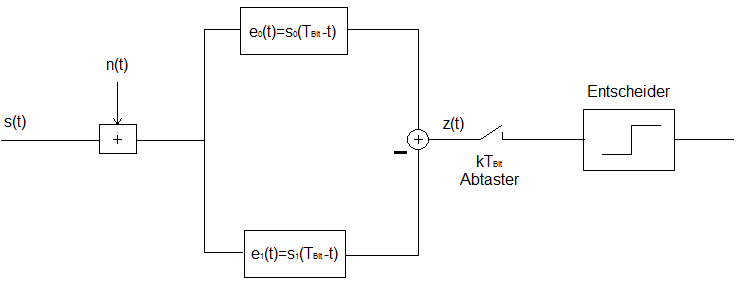
\includegraphics[scale=0.7]{Bilder/SAF-Filter}
        \caption{Kanal plus SAF}
        \label{fig:Kanal_pl_SAF}
    \end{figure}
     
    \end{quote}
    
   
\end{quote}

\section{Auswertung \& Theorie}
\begin{quote}
    
    \subsection{Encoderkennlinie}
    
    \begin{quote}
        
    
    
    \end{quote}
    
    
    \subsection{Quantisierungfehler}
    
    \begin{quote}
        
    \end{quote}    
    
\end{quote}

\section{Zusammenfassung}
\begin{quote}
	
	Es hat sich in diesem Versuch gezeigt, dass die Bitfehlerwahrscheinlichkeit bei der Übertragung mit Hilfe eines SAF
	deutlich von der Signalsendeform abhängt. Dabei ist eine Sendeform mit einer normierten Kruzkorrelation zwischen den
	Sendeimpulsen von -1 zu bevorzugen.
 
    
\end{quote} % end Sec: section


\end{document}
